	\documentclass[12pt,a4paper,twoside]{article}
\usepackage[ngerman]{babel}
\usepackage{amsmath}
\usepackage{amssymb}
\usepackage{graphicx}
\usepackage[utf8]{inputenc}
\usepackage[numbers,round]{natbib}
\usepackage{abschlussarbeit}
\usepackage{hyperref}
\usepackage{mathtools}
\usepackage{dsfont}
%\usepackage{ulem}
\usepackage{color}
%\usepackage{cite}
%\usepackage{natbib}
\setlength{\voffset}{-28.4mm}
\setlength{\hoffset}{-1in}
\setlength{\topmargin}{20mm}
\setlength{\oddsidemargin}{25mm}
\setlength{\evensidemargin}{25mm}
\setlength{\textwidth}{160mm}

\setlength{\parindent}{0pt}

\setlength{\textheight}{235mm}
\setlength{\footskip}{20mm}
\setlength{\headsep}{50pt}
\setlength{\headheight}{0pt}

\pagestyle{headings}
\bibliographystyle{authordate2}



\newtheorem{Satz}{Satz}[section]
% Ein sog. "Theorem" mit Abkuerzung "Satz" (das erste "Satz")
% Das zweite "Satz" bezeichnet den Namen des Theorems. (z.B. "Satz x.y" erscheint im TeX-File).
% [chapter] regelt die Numerierung der Saetze, in diesem Fall werden die Saetze pro Kapitel fortlaufend numeriert.

\newtheorem{Korollar}[Satz]{Korollar}
% Hier haben wir ein "Theorem" mit Abkuerzung "Korollar", welches im Tex-File als "Korollar" erscheint und in die "Theorem"-Nummerierung
% fortlaufend eingebunden wird (das "[Theorem]" bewirkt dies).
\newtheorem{Proposition}[Satz]{Proposition}
% Abkuerzung ist "Proposition", Name ist "Proposition", wird in "Theorem"-Nummerierung eingebunden.
%Lemma, ebenfalls in "Theorem"-Nummerierung eingebunden
\newtheorem{Lemma}[Satz]{Lemma}
%Definition, ebenfalls in "Theorem"-Nummerierung eingebunden
\newtheorem{Definition}[Satz]{Definition}
%Beispiel, ohne Nummerierung
\newtheorem{Beispiel}{Beispiel}
\newtheorem{Bemerkung}{Bemerkung}
\newtheorem{Beweis}{Beweis}

%Annahme, nach Kapiteln nummeriert
\newtheorem{Annahme}{Annahme}[section]
% Labelnummerierung in 'roemisch'.
\renewcommand{\labelenumi}{(\roman{enumi})}


\begin{document}
\pagestyle{empty}
%%%% Titelseite
\begin{titlepage}
\begin{center}

\includegraphics{TUMblau.png}\\[3mm]
\sf
{\Large
  Technische Universit"at M"unchen\\[5mm]
  Fakult"at f"ur Mathematik\\[8mm]
}
\normalsize

\includegraphics{MA_Web.png}\\[15mm]

Bachelor-Arbeit\\[15mm]

{\Huge
  Titel
}
\bigskip

\normalsize

Markus Stachl
\end{center}
\vspace*{75mm}

Aufgabensteller: ...
\medskip

Betreuer: ...
\medskip

Abgabetermin: ...

\end{titlepage}
%%%% Erklaerung - Unterschrift nicht vergessen!

\vspace*{150mm}

Ich erkl"are hiermit, dass ich die Bachelor-Arbeit selbst"andig und nur mit den angegebenen
Hilfsmitteln angefertigt habe.
\bigskip

Garching, den
\newpage
%%%% Zusammenfassung in englischer Sprache
\section*{Summary}
Bei einer in deutscher Sprache verfassten Arbeit muss eine Zusammenfassung in englischer Sprache vorangestellt werden.
Daf"ur ist hier Platz.

\newpage
\tableofcontents
\newpage

%%%% Ab hier beginnt die eigentliche Nummerierung der Seiten
\pagenumbering{arabic}
\pagestyle{headings}

\section{Inhalt}
Und los geht's
\begin{itemize}
	\item Optimale Kontrolle/Optimales Feedback (Einführung)
		\begin{itemize}
			\item set oriented approach
			\item Konstruktion der Wertefunktion
			\item Optimalitätsprinzip Bellman (Dynamic Programming (vgl \cite{mahoney2008}))
		\end{itemize}
	\item Niedrig-Rank-Approximation einer Matrix
		\begin{itemize}
			\item SVD
			\item CUR
			\item CX
			\item Vorteile Nachteile
		\end{itemize}
	\item CUR Decomp
		\begin{itemize}
			\item Rating der Spalten/Zeilen
			\item Algo
		\end{itemize}
	\item Ausblick: NNCUR NNCX
	\item Fallbeispiel invertiertes Pendel
\end{itemize}
\section{Einführung und Motivation}
	Die Vorarbeit und Basis zu dieser Arbeit besteht im Wesentlichen aus den beiden Papern...
	\subsection{Optimale Kontrolle}
	Gegeben sei das Problem der optimalen Stabilisierung eines (instabilen) diskreten Systems
	\begin{equation}
		x_{k+1}=f(x_k,u_k), \hspace{1,5cm} k=0...n
	\end{equation}
	um einen Fixpunkt $0\in X$, also $f(0,0)=0$. Der Fixpunkt kann o.B.d.A gewählt werden, ein anderer Fixpunkt kann 
	gegebenfalls in den Nullpunkt geshiftet werden. Die $x_k$ sind aus dem Zustandsphasenraum $X\subset \mathbb{R}^n
	$, die $u_k$ aus der Feedback-Menge $U\subsetneq \mathds{R}^m$. $X$ und $U$ sind jeweils kompakte Teilmengen der 
	Grundräume. Die Kosten pro Schritt sind dabei gegeben durch eine (stetige) Kostenfunktion $g: X\times U
	\rightarrow [0,\infty)$ mit $g(x,u)\geq 0 \hspace{0,2cm}\forall x\in X, u\in U$ und $g(x,u)=0 \Leftrightarrow 
	x=0, u=0$. \\
	Das Feedback $u$ soll nun so gewählt werden, dass die entstehenden Kosten minimiert werden und der Fixpunkt $0$ 
	zu einem asymptotisch stabilen Fixpunkt wird. Anders ausgedrückt: ausgehend von einem Punkt $x\in X$ soll ein
	Kontrollvektor $u=(u_1,u_2...)$ gewählt werden, sodass die Trajektorie 
	\begin{equation*}
		x_0(x,u)=x, \hspace{2cm} x_{k+1}=f(x_k(x,u),u_k=, k=0,1,...
	\end{equation*}
	für alle $k$ in $X$ verbleibt und $x_k(x,u)\rightarrow 0$ für $k\rightarrow\infty$ (vgl. \cite{Grune2005}). Alle Punkte $x$, für die eine Stabilisierung möglich ist werden in der Menge 
	\begin{equation*}
		S=\{x\in X| \exists u\in U^{\mathds{N}}: x_k(x,u)\rightarrow 0\}
	\end{equation*}
	zusammengefasst. \\
	Somit ergibt sich für die gesamten Kosten zur Stabilisierung eines Punktes $x\in X$ entlang einer Trajektorie
	\begin{equation}
		J(x,u)=\sum_{k=0}^{\infty}q(x_k(x,u),u_k) \hspace{1.5cm} \in [0,\infty]
	\end{equation}
	Ist $x$ nicht stabilisierbar, d.h. es existiert kein $u\in U^{\mathds{N}}$ sodass $x_k(x,u)\rightarrow 0$, so ist $J(x,u)=\infty$ und $x\in X\setminus S$. \\
	Gesucht sind nun die minimalen Kosten zur Stabilisierung (vgl. \cite{Junge2004}) eines Punktes $x$, die Kostenfunktion
	\begin{equation}
		\label{eq:valuefunction}
		V(x)=\inf_{u\in U^{\mathds{N}}}J(x,u)
	\end{equation}
	\subsection{Berechnung der Wertefunktion}
	Im Folgenden soll nun die zuvor definierte optimale Wertefunktion \ref{eq:valuefunction} numerisch berechnet werden. Hierzu wird das \textit{Optimalitätsprinzip nach Bellman} (vgl. \cite{deuflhard2008}) zu Hilfe genommen:
	\begin{equation}
		\label{eq:bellman}
		V(x)=\inf_{u\in U^{\mathds{N}}}\{q(x,u)+V(f(x,u)\}
	\end{equation}
	wobei sich die optimale Steuerungssequenz ergibt aus
	\begin{equation}
		u(x)=argmin_{u\in U^{\mathds{N}}}\{q(x,u)+V(f(x,u)\}
	\end{equation}
	Zur numerischen Lösung dieses Optimierungsproblems wird ein Ansatz aus der Graphentheorie gewählt: \\
	Die (kompakte) Menge $X$ wird partitioniert, d.h. es entsteht eine Menge $\mathcal{P}$
	von Teilmengen $P_i\subset X, i=1,...,l,$ wobei $\cup_{i=1}^lP_i=X$ und $m(P_i \cap P_j)=0$ für $i\neq j$ ($m$ 
	bezeichnet hier das Lebesque-Maß). \\
	Auf dieser Partition wird nun ein gerichteter Graph 
	\begin{equation*}
		G_\mathcal{P}=(\mathcal{P},E_\mathcal{P}), \hspace{2cm} E_\mathcal{P}=\{(P_i,P_j)\in \mathcal{P}\times \mathcal{P} \hspace{2mm}|\hspace{2mm}f(P_i,U)\cap P_j\neq \emptyset\}
	\end{equation*}
	definiert. Hierbei sind die Gewichte der Kanten $e=(P_i,P_j)$ (vgl. \cite{Junge2004}) alle nichtnegativ und 
	gegeben durch
	\begin{equation*}
		w(e)=\min_{x\in P_i, u\in U}\{q(x,u)|f(x,u)\in P_j\}.
	\end{equation*}
	Bild 1 zeigt schematisch solch einen Graphen ausgehend von einem Punkt $x$.
	\vspace{1cm}
	\\
	Bild des Graphen
	\vspace{1cm}
	\\
	Anstatt der exakten Wertefunktion $V(x)$ (\ref{eq:bellman}) wird nun die approximative Wertefunktion
	\begin{equation*}
		V_\mathcal{P}(x)=\min\{w(p(x)) \hspace{2mm}|\hspace{2mm} \text{Pfad}\hspace{1mm} p(x)=(e_1,...,e_m), e_k\in E_\mathcal{P} \hspace{1mm}\text{verbindet x mit dem Ursprung}\}
	\end{equation*}
	berechnet. \newline
	\newline
	Um, ausgehend von dem bestimmten Graphen, den kürzesten Weg und damit die bestmögliche Stabilisierung bezüglich 
	der Kosten zwischen einem Punkt x und einem Fixpunkt $0$ zu bestimmen, können Standard-\textit{shortest-path}-Algorithmen wie beispielsweise der Algorithmus von Dijkstra (vgl. \citep{Dijkstra59}) verwendet werden.
	\newline
	Somit kann für jedes Element der Partition $\mathcal{P}$ eine optimale Stabilisierung, d.h. bezüglich der geringsten Kosten, berechnet werden. \newline
	\newline
	\textbf{Konvergenz:} Für alle Punkte $x\in S$, für die eine Stabilisierung möglich ist, und für den Partitionsdurchmesser $diam(\mathcal{P}):=\max_i\{diam(P_i)\}\rightarrow 0$ gilt:
	\begin{equation*}
		V_\mathcal{P}(x)\rightarrow V(x)
	\end{equation*}
	Für einen Beweis siehe \cite{Junge2004}. \\
	Schreibt man den resultierenden Boxplot in Matrixform, erhält man Folgendes: \\
	\begin{figure}[h]
		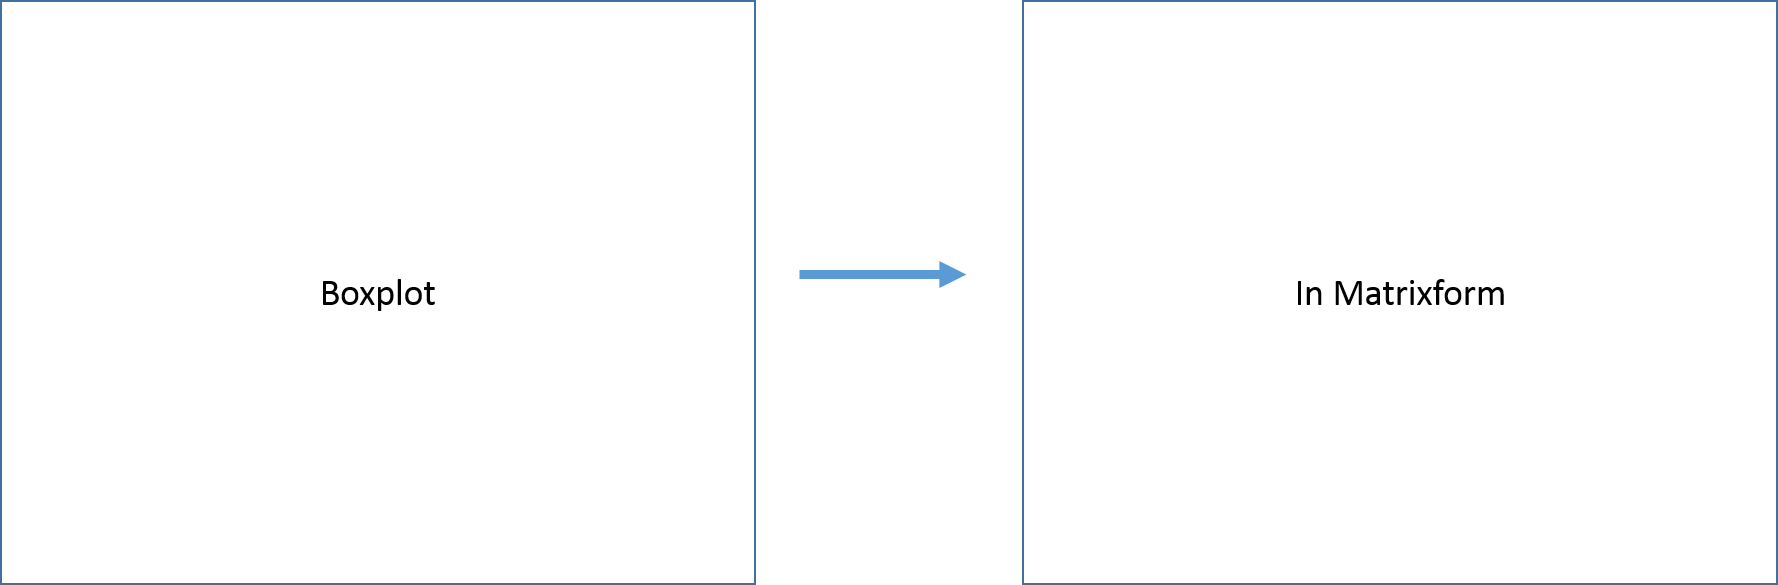
\includegraphics[scale=0.5]{testbild}
		\caption{Umformung des Boxplots in Matrixform}
	\end{figure}
	\\
Da diese Matrizen je nach Parameter ziemlich groß werden können, sollen sie approximiert werden. Im nächsten Kapitel werden diverse Approximationsmethoden vorgestellt.
\section{Niedring-Rang-Appriximation einer Matrix}
	Je nach Tiefe der Simulation bzw. der Dimension des zugrunde liegenden Raumes (vgl. Fluch der Dimension \textbf{Bellman}) können gigantische Matrizen entstehen. Da die gängigen Rechner bei der Speicherung solcher Matrizen schnell an ihre Grenzen stoßen, soll nun für die Wertematrix $V$ eine Niedrig-Rang-Approximation der Form
	\begin{equation}
		\label{eq:approx}
		V(x)\approx \sum_{i=1}^k\sigma_i u_i(x) v_i^T(x)
	\end{equation}
	gefunden werden, wobei $\sigma_i\in \mathds{R}$ Konstanten und $u_i, v_i$ Vektoren im $\mathds{R}^n$ sind. Im Folgenden werden einige Näherungen vorgestellt.
	\subsection{Singulärwertzerlegung (SVD)}
		Dies klassische Singulärwertzerlegung .... ... und ist folgendermaßen definiert.		
		\begin{Definition}
		Sei A eine komplexe $m\times n$-Matrix von Rang $r$. Die Singulärwertzerlegung von A ist gegeben durch (vgl. 			\cite{deuflhard2008})
		\begin{equation*}
			\label{eq:SVD}
			A=U\Sigma V^* 
		\end{equation*}
		wobei
		\begin{itemize}
			\item $U$ eine unitäre $m\times m$-Matrix ist,
			\item $V^*$ die Adjungierte einer $n\times n$-Matrix $V$ ist und
			\item $\Sigma$ eine reelle $m\times n$-Diagonalmatrix der Form \[
	 		\Sigma = \left(\begin{array}{ccc|ccc}
					\sigma_1 &          &         &       & \vdots &       \\
         			& \ddots   &         & \cdots & 0      & \cdots \\
         			&      &\sigma_r &        & \vdots &        \\
					\hline
        			 &  \vdots  &        &       & \vdots &        \\
					\cdots   & 0       & \cdots   & \cdots & 0      & \cdots \\
        			 &  \vdots  &         &        & \vdots &        \\
					\end{array}\right)
			\]
			Die Einträge $\sigma_i>0$, $i=1...r$, $\sigma_1>...>\sigma_r$ heißen Singulärwerte von A. Die Spalten von $U$, $u_i$, heißen linke Singulärvektoren, die Spalten von $V$, $v_i$, heißen rechte Singulärvektoren.
		\end{itemize}
		\end{Definition}
		\begin{Bemerkung}
			$A$ kann auch geschrieben werden als die Summe von Rang-1-Matrizen:
			\begin{equation*}
				\label{eq:SVDsum}
				A=\sum_{i=1}^r\sigma_i u_i v_i^T
			\end{equation*}
			Die $\sigma_i$ sind dabei die Singulärwerte von $A$ und $u_i$ und $v_i$ die Zeilen von $U$ bzw. $V$.
		\end{Bemerkung}
		Die Berechnungskosten, die für das Ausführen der Matrixzerlegung benötigt werden, betragen $\mathcal{O}(min(mn^2,m^2n))$ (vgl \cite{mahoney2008}).
		\newline 
		\newline
		Wir wollen die Wertematrix $V$ nun so approximieren, dass der Fehler 
		\begin{equation*}
			e(D)=||V-D||_\xi
		\end{equation*}
		bezüglich einer Norm $\xi$ möglichst klein wird für Matrizen $D$ von Rang $rank(D)\leq k$. $\xi=2$ bezeichnet hierbei die 2-Norm ($||A||_2=\left(\sum_{i,j}|a_{ij}|^2\right)^\frac{1}{2}$), $\xi=max$ bezeichnet die Maximumsnorm ($||A||_{max}=\max_{i,j}|a_{ij}|$) und $\xi=F$ verwendet die Frobeniusnorm ($||A||_F=(\sigma_1^2+...+\sigma_r)^\frac{1}{2}$).
		\newline
		\newline
		Die erste Frage, die auftaucht: gibt es eine "beste" Rang-k-Approximation.
		\begin{Satz}{(Eckart-Young)}
			Sei eine Matrix $V$ von Rang $r$ gegeben durch \ref{eq:SVD} und $k<r$. Die beste Rang-$k$-Approximation 
			von $V$, also eine Matrix, die
			\begin{equation*}
				\min_{rank(B)\leq k}||V-B||_2	
			\end{equation*}		
			erfüllt, ist gegeben durch
			\begin{equation*}
				 V_k=\sum_{i=1}^k\sigma_i u_i v_i^T
			\end{equation*}
			und 
			\begin{equation*}
				||V-V_k||_2=\sigma_{k+1}
			\end{equation*}
			wobei $\sigma_{k+1}$ der (k+1)-te Singulärwert von $V$ ist. Dies impliziert, dass für Singulärwertzerlegungen von Rang $k\geq r$ gilt: $||V-V_k||_2=0$.
		\end{Satz}
		\begin{Beweis}
			Für einen Beweis siehe \cite{Golub2013}.
		\end{Beweis}
		Die Kosten der k-Rang-Singulärwertzerlegung betragen $\mathcal{O}(mnk)$ \citep{Wang2013}. \newline
		\newline
		\textbf{Nachteil:} Es werden keine konkreten Einträge der ursprünglichen Matrix $V$ verwendet, deswegen......\newline
		\newline
		In den nächsten beiden Abschnitten werden zwei Verfahren vorgestellt, welche Spalten und/oder Zeilen der 
		Eingabematrix verwenden.
	\subsection{CX-Zerlegung}
		\label{subsec:CX}
		Die erste approximative Matrix-Zerlegung, welche konkrete Einträge der ursprünglichen Matrix verwendet, ist die CX-Zerlegung (vgl. \citep{Drineas2009}). 
		\begin{Definition}
			Sei $A$ eine $m\times n$-Matrix. Sei $C\in \mathds{R}^{m\times c}$ eine Matrix bestehend aus $c$ Spalten der Matrix A (in der Regel ist $c\ll n$). Dann ist die approximative Matrix $A'=CX$ für jede beliebige Matrix $X\in \mathds{R}^{c\times n}$ eine spaltenbasierte Approximation von $A$, beziehungsweise eine $CX$-Zerlegung von $A$.
		\end{Definition}
	\subsection{CUR-Zerlegung}	
		\label{subsec:CUR}
		Bei der CUR-Zerlegung werden im Gegensatz zur CX-Zerlegung Spalten und Zeilen der zu approximierenden Matrix 
		verwendet. Die Matrix C enthält dabei Spalten von $V$ und Zeilen werden in R gefasst. Die Matrix $U$ wird 
		dann so gewählt, dass der Fehler zwischen V und CUR bezüglich einer Norm minimal wird. \\
		Die mathematische Definition der CUR-Zerlegung ist wiefolgt:
		\begin{Definition}{(vgl. \citep{Drineas2009})}
			Gegeben sei eine Matrix $V\in \mathds{R}^{m\times n}$. Sei $C\in\mathds{R}^{m\times 
			c}$ eine Matrix, welche aus $c$ Spalten von $V$ besteht, und $R\in\mathds{R}^{r\times n}$ eine Matrix, 
			deren $r$ Zeilen aus Zeilen von $V$ bestehen. Dann ist die Matrix $V'=CUR$ für jede beliebige Matrix $U
			\in\mathds{R}^{c\times r}$ eine Spalten-Zeilen-basierte Approximation von $V$, beziehungsweise eine $CUR
			$-Zerlegung von $V$.
		\end{Definition}
		Im Folgenden wird ein Verfahren zur Berechnung der $CUR$-Zerlegung von Mahoney und Drineas \citep{mahoney2008} vorgestellt. \newline
		\newline
		Besonders kritisch bei der Berechnung der Zerlegung ist, welche Zeilen bzw. Spalten für die Approximation 
		verwendet werden.
		Dafür wird ein Rating erzeugt (siehe \citep{mahoney2008}), welche den Einfluss einer Spalte/Zeile auf die 
		restlichen Einträge der Matrix beschreibt. \newline
		\newline	
		\textbf{Bestimmung des statistischen Einflusswertes einer Spalte/Zeile:} \newline 
		Aus \ref{eq:SVDsum} wissen wir, dass sich die $j$-te Spalte einer Zielmatrix $V$ von Rang $r$ darstellen lassen kann als
		\begin{equation*}
			V^j=\sum_{\xi=1}^r(\sigma_\xi u^\xi )v_j^\xi
		\end{equation*}
		bzw. deren "beste" \ Rang-k-Approximation durch
		\begin{equation*}
			V^j=\sum_{\xi=1}^k(\sigma_\xi u^\xi )v_j^\xi
		\end{equation*}
		wobei $u^\xi$ der $\xi$-te linke Singulärvektor und $v_j\xi$ die $j$-te Koordinate des $\xi$-ten rechten 
		Singulärvektors ist. Der statistische Einflusswert einer Spalte von $V$ kann nun gemessen werden durch
		\begin{equation}
			\label{eq:score}
			\pi_j=\frac{1}{k}\sum_{\xi=1}^k(v_j^\xi)^2 \hspace{2cm} j\in [1,n]
		\end{equation}
		Diese Einflusswerte bilden eine Wahrscheinlichkeitsverteilung auf den $n$ Spalten und es gilt: $\sum_{j=1}^n\pi_j=1$ und $\pi_j\geq 0$ \newline
		Das Selektieren der Spalten wird anschließend mithilfe des Algorithmus' COLUMNSELECT (vgl. \citep{mahoney2008}) durchgeführt: \newline
		\begin{enumerate}
			\item \textbf{Input:} Matrix $V\in \mathds{R}^{m\times n}$ und Fehlerparameter $\epsilon$
			\item Berechne die ersten $k$ rechten Singulärvektoren ($v_1,...,v_k$) von V und die statistischen Einflusswerte \ref{eq:score} der Spalten von V.
			\item Verwende die $j$-te Spalte von V mit Wahrscheinlichkeit $p_j=min\{1,c\pi_j\}$, wobei $c=\mathcal{O}(k \log \frac{k}{\epsilon^2})$
			\item \textbf{Output:} Matrix $C$, welche aus den selektierten Spalten von $A$ besteht.
		\end{enumerate}
		Mithilfe dieses Algorithmus' entsteht eine Matrix $C$, die $c'\leq c$ der selektierten Spalten verwendet. Die 
		Kosten zur Ausführung des Algorithmus' beruhen hauptsächlich auf der Berechnung der ersten $k$ 
		Singulärvektoren und sind daher $\mathcal{O}(mnk)$ \citep{mahoney2008}.\newline
		Zur Berechnung der Vektoren $C,U$ und $R$ wird abschließend folgender Algorithmus ALGORITHMCUR (vgl \citep{mahoney2008}) verwendet:
		\begin{enumerate}
			\item Wende COLUMNSELECT auf $A$ an mit $c=\mathcal{O}(k \log \frac{k}{\epsilon^2})$ und berechne somit die Matrix $C$
			\item Wende COLUMNSELECT auf $A^T$ an mit $r=\mathcal{O}(k \log \frac{k}{\epsilon^2})$ und berechne somit die Matrix $R$
			\item Definiere die Matrix $U$ als $U=C^+AR^+$, wobei $X^+$ die Moore-Penrose-Inverse von X ist
		\end{enumerate}
		Die so konstruierte approximative Matrix $V'=CUR$ erfüllt nun, dass
		\begin{equation*}
			||V-V'||_F\leq (2+\epsilon )||V-V_k||_F
		\end{equation*}		
		mit hoher Wahrscheinlichkeit (m.h.W.) (vgl. \citep{mahoney2008}). \newline
		\newline
		Die Rate $(2+\epsilon)$ kann mit einer Variation des Algorithmus' noch weiter verbessert werden \citep{Drineas2009}. Bei dieser Methode wird die Matrix $R$ abhängig von den für die Matrix $C$ gewählten Zeilen berechnet. Durch diese Abwandlung verringert sich der Fehler m.h.W. zu
		\begin{equation*}
			||V-CUR||_F\leq (1+\epsilon)||V-V_k||_F
		\end{equation*}
		Dies ist nur eine Möglichkeit eine approximative $CUR$-Zerlegung der Matrix $V$ zu finden. Weitere werden in 
		folgender Tabelle gezeigt: \newline
		\begin{figure}[h]
			\begin{tabular}{l||c|c|c|c}
		 		& Anzahl Spalten c & Anzahl Reihen r & rank(U) & $||V-CUR||_F^2\leq$ \\
		 		\hline \hline
		 		Drineas et al. 2003 \citep{drineas2003} & $\frac{k}{\epsilon^2}$ & $\frac{k}{\epsilon^2}$ & $k$ & $||V-V_k||_F^2+\epsilon||A||^2_F$ \\
		 		\hline
		 		Drineas et al. 2008 \citep{Drineas2009} & $\frac{k\log k}{\epsilon^2}$ & $\frac{k\log k}{\epsilon^4}$ & $\frac{k\log k}{\epsilon^2}$ & $(1+\epsilon)||V-V_k||^2_F$ \\
		 		\hline
		 		Wang et al. 2013 \citep{Wang2013}& $\frac{k}{\epsilon}$ & $\frac{k}{\epsilon^2}$ & $\frac{k}{\epsilon}$ & $(1+\epsilon)||V-V_k||^2_F$
			\end{tabular}
			\caption{Tabelle über verschiedene CUR-Approximationen}
		\end{figure}
		
		\textbf{Vorteil:} Zeilen und Spalten der ursprünglichen Matrix werden verwendet  \newline
		\newline
		\textbf{Nachteil:} Die approximierende Matrix ist nicht mehr von der Form \ref{eq:approx}. \newline
		\newline
	
	\newpage
\section*{Abkürzungen}
	\begin{tabular}{ll}
		SVD & Singulärwertzerlegung \\
		m.h.W. & mit hoher Wahrscheinlichkeit \\
	\end{tabular}
\newpage
\bibliography{BA_lib}
\end{document}
